\documentclass[11pt,a4paper,dvipsnames,twosided]{article}

\usepackage[deliverable]{IOHKCoverPage}

% data for Deliverable header -- added by KH from an EU H2020 project template
\DeliverableNumber{SL-D1}
\DeliverableTitle{A Specification of the Non-Integral Calculations \\ in the Shelley Ledger}{Non-Integral Cals.}
\DeliverableResponsible{Formal Methods Team}
\EditorName{Matthias G\"udemann, \IOHK}
\Authors{Matthias G\"udemann \quad \texttt{<matthias.gudemann@iohk.io>}
}
\DueDate{20$^{\textrm{th}}$ September 2019}
\SubmissionDate{18$^{\textrm{th}}$ September 2019}{2019/09/18}
\LeaderName{Philipp Kant, \IOHK}
\InstitutionAddress{\IOHK}
\Version{0.2}
\Project{Shelley Ledger}
\DisseminationDR

\usepackage[margin=2.5cm]{geometry}
\usepackage{lscape}
\usepackage{iohk}
\usepackage{microtype}
\usepackage{mathpazo} % nice fonts
\usepackage{amsmath}
\usepackage{amssymb}
\usepackage{amsthm}
\usepackage{latexsym}
\usepackage{mathtools}
\usepackage{subcaption}
\usepackage{stmaryrd}
\usepackage{extarrows}
\usepackage{slashed}
%\usepackage[colon]{natbib}
\usepackage[unicode=true,pdftex,pdfa,colorlinks=true]{hyperref}
\usepackage{xcolor}
\usepackage[capitalise,noabbrev,nameinlink]{cleveref}
\usepackage{float}
\floatstyle{boxed}
\restylefloat{figure}
\usepackage{tikz}

%% Commenting -- KH
\usepackage[final,obeyFinal]{todonotes}
\newcommand{\khcomment}[1]{\todo[color=blue!20]{KH: #1}}

%% In-para enumeration -- KH
\usepackage{paralist}

%%
%% Package `semantic` can be used for writing inference rules.
%%
\usepackage{semantic}
%% Setup for the semantic package
\setpremisesspace{20pt}

\newcommand{\unitInterval}{\ensuremath{[0,~1]}}
\newcommand{\nonnegReals}{\ensuremath{[0,~\infty)}}
\newcommand{\posReals}{\ensuremath{(0,~\infty)}}

\theoremstyle{definition}
\newtheorem{definition}{Definition}[section]

\theoremstyle{definition}
\newtheorem{property}{Property}[section]

\begin{document}

\hypersetup{
  pdftitle={A Specification of the Non-Integral Calculations in the Shelley Ledger},
  breaklinks=true,
  bookmarks=true,
  colorlinks=false,
  linkcolor={blue},
  citecolor={blue},
  urlcolor={blue},
  linkbordercolor={white},
  citebordercolor={white},
  urlbordercolor={white}
}

  \cleardoublepage%
  \tableofcontents%
  \listoffigures%
  \clearpage%

  \begin{changelog}
        \change{05/09/19}{Matthias G\"udemann}{FM (IOHK)}{Initial version (0.1).}
        \change{05/09/19}{Kevin Hammond}{FM (IOHK)}{Reviewed and applied comments.}
        \change{12/09/19}{Kevin Hammond}{FM (IOHK)}{Added cover page for consistency.}
        \change{12/09/19}{Kevin Hammond}{FM (IOHK)}{Included review comments from MG.}
        \change{17/09/19}{Matthias G\"udemann}{FM (IOHK)}{Reviewed and commented.}
        \change{18/09/19}{Kevin Hammond}{FM (IOHK)}{MG comments incorporated, added deliverable number, frozen to V0.2}
\end{changelog}
\begin{landscape}
\floatstyle{plain}
\restylefloat{figure}
\begin{figure*}
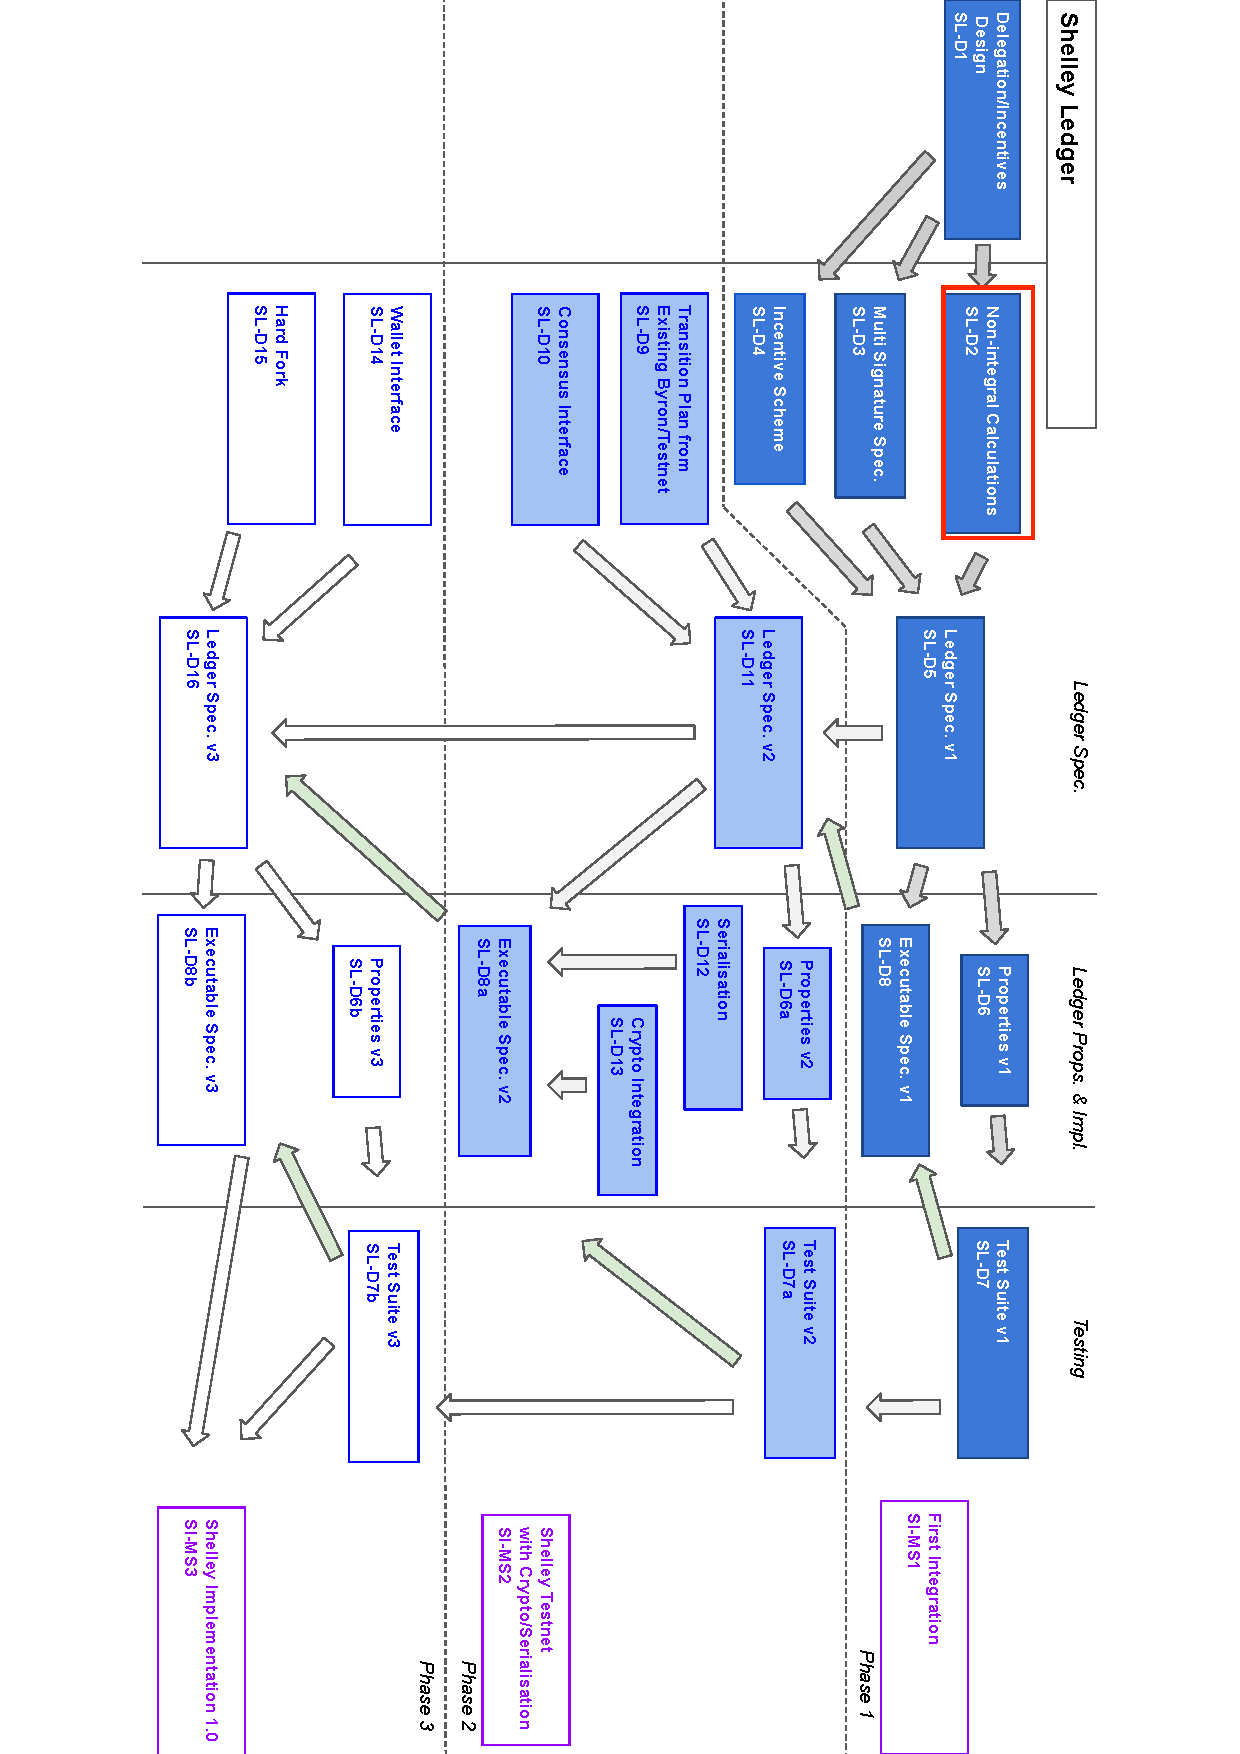
\includegraphics[scale=0.8,angle=90]{d2-depends.pdf}
\caption{Positioning of this Deliverable (outlined in red).}
\end{figure*}
\end{landscape}
%\floatstyle{boxed}
\restylefloat{figure}
\pagestyle{empty}

\cleardoublepage
\renewcommand{\thepage}{\arabic{page}}
\setcounter{page}{1}

\title{A Specification of the Non-Integral Calculations in the Shelley Ledger}

\author{Matthias G\"udemann  \\ {\small \texttt{matthias.gudemann@iohk.io}}}

%\date{}

\maketitle

\begin{abstract}
  This document defines a consistent way to perform non-integral calculations in
  the Shelley ledger for Cardano. These calculations are defined in terms of
  \emph{elementary} mathematical functions, and are used in a few, but
  important, places in the ledger calculation.  The main objective of this work
  is to provide a clear and unambiguous specification that will give the same
  results for each calculation, regardless of the computer architecture or
  programming language implementation that is chosen.  The goal is to prevent
  blockchain forks because of slight differences in the calculated values that
  might otherwise come from different implementations of the Shelley ledger
  specification or Ouroboros protocol, for example.
\end{abstract}

\tableofcontents
\listoffigures

\section{Introduction}
\label{sec:introduction}

The Shelley ledger specification~\cite{shelley_spec} and the Ouroboros
protocol~\cite{ouroboros} use non-integral calculations in a few places. Most of
these can be implemented in an exact way using rational numbers and arbitrary
precision integers, which are available either directly as programming language
constructs (e.g. in Haskell) or via external libraries.~ \footnote{The most
  widely used library is the GNU multi-precision library (GMP)}
%
In addition, there are some instances where the results of elementary functions
cannot be precisely represented as rational numbers, and therefore require a
representation that covers a wider range of \emph{real numbers}.  These include
the exponential function $e^{x}, x \in \mathbb{R}$, which is used to calculate
how refunds decay over time, and general non-integral exponentiation
$x^{y}, x, y \in \mathbb{R}$. %, which is used to \khcomment{MG, please fix!}.

\section{Problem Description}
\label{sec:problem-description}

The calculations in the Shelley ledger specification and Ouroboros protocol that involve elementary functions are concerned with:
\begin{inparaenum}
\item
  the decay of the value that should be refunded from a deposit;
and
\item
  the leader election probability.
\end{inparaenum}
%
In all these cases, it is important that all distributed nodes calculate the
same values, since otherwise there might be a disagreement about what should be
included in the blockchain and forks might then result. This is a particular
problem where there could be multiple independent implementations that could
deliver inconsistent results.  Since Cardano aims to be a cryptocurrency that is
fully defined by a precise specification, we need an exact specification of
non-integer calculations, allowing different implementations to have the same,
correct and verifiable,
behavior.

\section{Implementation Possibilities for Non-Integer Arithmetic}
\label{sec:impl-poss}

There are three main different possibilities to implement non-integral
calculations. In Haskell, we can use typeclasses or parametric polymorphism
to design generic algorithms that can handle different choices. Each implementation choice has its
own advantages and disadvantages.

\subsection{IEEE~754 Floating Point}
\label{sec:ieee-754-floating}

A straightforward approach is to use IEEE~754 floating-point arithmetic.  This is
widely supported by common programming languages and CPU/GPU architectures.
%
The basic arithmetic operations of IEEE~754 floating-point are well specified,
and they are usually very efficient due to direct HW implementation.
%
Double-precision IEEE~754 floating-point numbers (\emph{binary64}) provide 53 bits (~15.99 decimal digits) of
precision.  This is slightly less than is needed to represent the
required fraction of 1 lovelace: there are $4.5\cdot10^{16}$ possible fractions.
Moreover, the  elementary functions that are required for Cardano are not standardized and there can be
subtle differences in different implementations, with results even varying when different compiler settings are used
on the same implementation\footnote{e.g. maintaining intermediate representations within internal registers \emph{vs.} writing to memory.}. It is also worth noting that some architectures
provide excess precision~\footnote{The original x87 provided 80 bit
  floating-point}, which can result in greater accuracy, but can also give slight differences in results
between implementations. Some programming languages, e.g., D, exploit this by default. Many
languages support excess precision, but default to IEEE~754 64 bits. In
particular on the AMD64 architecture most language implementations use SSE floating-point arithmetic.
A final problem is that IEEE~754 supports different rounding modes\footnote{round to nearest (with even digits breaking ties or ties rounding away from zero), round down, round up, round to zero},  which will obviously give
different results in some cases.  Some programming languages allow the rounding mode to be changed, e.g. C99 onwards, but others do
not, e.g., Haskell.

\subsection{Rational Numbers}
\label{sec:rational-numbers}

Rational numbers can be implemented on top of exact arbitrary precision integral
arithmetic using a pair of numbers to represent a numerator and denominator.
Effectively, \emph{gcd} calculations are used to normalize the results
after each basic operation. While not all real numbers are rationals, this approach allows for
arbitrarily precise approximation of all real numbers. However, arbitrarily
long numerators or denominators may be needed to represent irrational numbers to the required precision.
These arbitrarily long numerators and denominators are undesirable, since they will incur non-predictable~\footnote{potentially > 1s for basic arithmetic operations}
run-time.

\subsection{Fixed Point Arithmetic}

%% KH: added this discussion
Fixed point arithmetic uses a fixed size value (typically 32 or 64 bits) to
represent non-integer numbers.  A fixed scaling factor is used to determine the
position of the decimal point and normal integer arithmetic operations are
applied for addition, multiplication etc.  Like floating point, this has the
advantage of allowing a compact number representation, and allows fast implementation even on
a system without floating point supprt.  It also allows precise arithmetic.  However,
arbitrarily large numbers cannot be supported, which would make it unsuitable for
representing currency in Cardano (it might, however, be suitable for e.g. leader election calculations).


\subsection{Fixed Precision Arithmetic}
\label{sec:fixed-point-arithm}

An alternative approach is to use fixed precision arithmetic based on exact
integers where a proportion of the integer is used as fractional part.  The
number of fractional digits is fixed to a constant.  This is more efficient than
using the rational number approach described above, since it is not necessary to
normalise values after calculations, arbitrary precision results are not
supported, and only a single arbitrarily sized integer needs to be stored.
Since it is implemented purely in software on top of exact integer arithmetic,
this approach will be less efficient than IEEE~754 floating point.  However, it
can be made to behave equivalently in different implementations, including
ensuring consistent (bounded) timings for each architecture, by providing golden
tests to validate consistent esults for different architectures etc.

The basic idea is the following: for $n$ decimal digits of precision, multiply
each integral value by $10^{n}$ and take this into account in the basic
operations. For Cardano, this would mean using $n=17$ to support the required 17
digits of precision that would track each possible stake fraction.  Haskell
provides library support for fixed precision numbers and arithmetic.

\subsection{Exact Real Numbers}

Finally, there has been some research work on exact representations of real
numbers using e.g. \emph{continued fractions}, exploiting lazy evaluation to
produce the required number of digits of precision
(e.g. \cite{DBLP:journals/tcs/Escardo96}).  All real numbers can be represented,
whether rational or irrational.  These approaches have not yet been widely used,
however, except for research purposes.  Implementations are often complicated
and expensive, and some algorithms may need to be changed (for example, exact
equality may be impossible to determine in a finite time).

\subsection{Conclusion}
\label{sec:summary}

For the Cardano cryptocurrency, the fixed precision arithmetic approach
seems to be most suitable. It allows for the desired precision and can be
implemented in an equivalent way, because it uses exact integer
arithmetic.~\footnote{There already exist two implementations, Haskell and C.}
While the fixed-precision approach is less efficient than IEEE~754 floating point,
by using partial pre-computation and other techniques, it will be possible to improve performance considerably in
some cases (e.g. when using a constant base for exponentiation): experiments show that improvements
of two orders of magnitude are possible.

\section{Approximation Algorithms}
\label{sec:algorithms}

Other than basic arithmetic (addition, multiplication, subtraction, and
division), the only elementary functions that are required by the ledger
specification are the exponential function, $e^{x}$, and its generalisation to
the exponentiation function, $x^{y}$. Exponentiation of arbitrary real numbers
is calculated using the identity:
$x^{y}= \exp({\ln(x^{y})}) = \exp(y\cdot \ln(x))$. This means that we need
suitable approximation schemes for $\exp(x)$ and $\ln(x)$.
%
There are two main approaches that are used for approximation: Taylor / MacLaurin series and
continued fractions. Both require only basic arithmetic operations and allow for
iterative approximation, i.e., constructing a sequence of $x_{0},x_{1},\ldots
x_{n}$ where each successive $x_{i}$ is a better
approximation to the desired value.

\subsection{Taylor Series}
\label{sec:taylor-series}

A Taylor series defines an infinite series that approximates an infinitely
differentiable function around a point $a$. It has the following general
form for a function $f$:

\begin{equation*}
  Tf(x; a) := \sum_{n=0}^{\infty}\frac{f^{(n)}(a)}{n!}
  {\left(
    x - a
  \right)}^{n}
\end{equation*}

Most commonly the Taylor series is used at $a=0$. This is also called the
MacLaurin series.  It uses a truncated, finite polynomial for the function
approximation as follows:

\begin{equation*}
  x_{m} := \sum_{n=0}^{m}\frac{f^{(n)}(0)}{n!} x^{n}
\end{equation*}

Using the above, the exponential function can be approximated using the Taylor series
by:

\begin{equation*}
  \exp(x) := \sum_{n=0}^{\infty}\frac{x^{n}}{n!}
\end{equation*}

The natural logarithm can similarly be approximated by:

\begin{equation*}
  \ln(x) := \sum_{n=1}^{\infty}\frac{(-1)^{n+1}}{n}
    {\left(
        x - 1
    \right)}^{n}
\end{equation*}

\subsection{Continued Fractions}
\label{sec:continued-fractions}

Continued fractions are a way to represent a number as the sum of its integral
part and the reciprocal of another number. The most general form looks like
this:

\begin{equation*}
  b_{0} + \cfrac{a_{1}}{b_{1} + \cfrac{a_{2}}{b_{2}  + \cfrac{a_{3}}{\ddots}}}
\end{equation*}

The convergents $x_{i} = \frac{A_{i}}{B_{i}}$ are computed via the following
recursion:

\begin{align*}
  A_{-1} & :=  1 \\
  A_{0} & :=  b_{0} \\
  B_{-1} & :=  0 \\
  B_{0} & := 1 \\
  A_{n} & :=  b_{n}\cdot A_{n-1} + a_{n}\cdot A_{n-2} \\
  B_{n} & :=  b_{n}\cdot B_{n-1} + a_{n}\cdot B_{n-2}
\end{align*}

For the exponential function $\exp(x)$, the sequences of $a_{i}$ and $b_{i}$ are
as follows:

\begin{align*}
  \sigma(a_{i}) & := 1 \cdot x, -1 \cdot x, -2 \cdot x, \ldots \\
  \sigma(b_{i}) & := 1, 2 + x, 3 + x, \ldots
\end{align*}

For the natural logarithm $\ln(x+1)$, the sequences of $a_{i}$ and $b_{i}$ are
as follows:

\begin{align*}
  \sigma(a_{i}) & := x, 1^{2}\cdot x, 1^{2}\cdot x, 2^{2}\cdot x, 2^{2}\cdot x, 3^{2}\cdot
          x, 3^{2}\cdot x, \ldots\\
  \sigma(b_{i}) & := 1, 2, 3, \ldots
\end{align*}

\subsection{Scaling}
\label{sec:scaling}

Neither Taylor series approximations nor continued fractions converge for arbitrary input
values: their convergence radius is limited. Therefore, we apply scaling before
we do the approximation, using the mathematical properties of $\exp$ and $\ln$
to obtain the correct results.

To calculate the exponential functions, we scale $x$ in such a way that
$x \in [0; 1]$ via:

\begin{equation*}
  \exp(x) = \exp
  \left(
    \frac{x}{n}\cdot n
  \right) =
  {\left(
      \exp{
        \left(
          \frac{x}{n}
        \right)}
    \right)}^{n}, \text{ with } n := \lceil x \rceil
\end{equation*}

For the natural logarithm, we calculate $n$ in such a way that
$\exp(n) \leq x < \exp(n+1)$ and use this as follows:

\begin{equation*}
  \ln(x) = \ln
  \left(
    \exp(n) \cdot \frac{x}{\exp(n)}
  \right) = \ln(\exp(n)) + \ln
  \left(
    \frac{x}{\exp(n)}
  \right) = n + \ln
  \left(
    \frac{x}{\exp(n)}
  \right)
\end{equation*}

This guarantees that $\frac{x}{\exp(n)}$ is in the interval $[1; e]$, which lies
in the convergence radius of the approximation schemes.

\subsection{Convergence}
\label{sec:convergence}

Our experimental results have shown that continued fractions converge faster, in particular for the natural logarithm.

\khcomment{Give captions for the plots.  Combine the plots from Figs. 1 and 2 into a single figure (one above the other?).  Do the same for Figs. 3 and 4.}

\begin{figure}[ht]
  \centering
    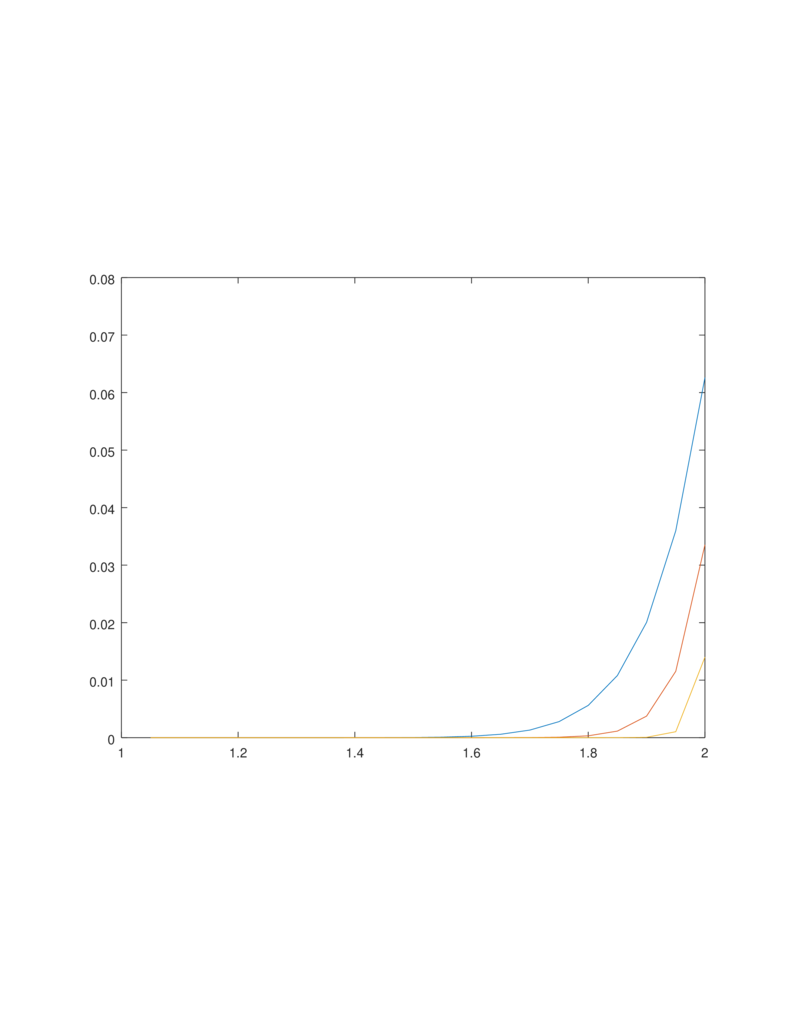
\includegraphics[width=\textwidth]{ln_taylor}
  \caption{Relative Error for Taylor Series Approximation of  $\ln$}
  \label{fig:ln-approx-taylor}
\end{figure}

\begin{figure}[ht]
  \centering
    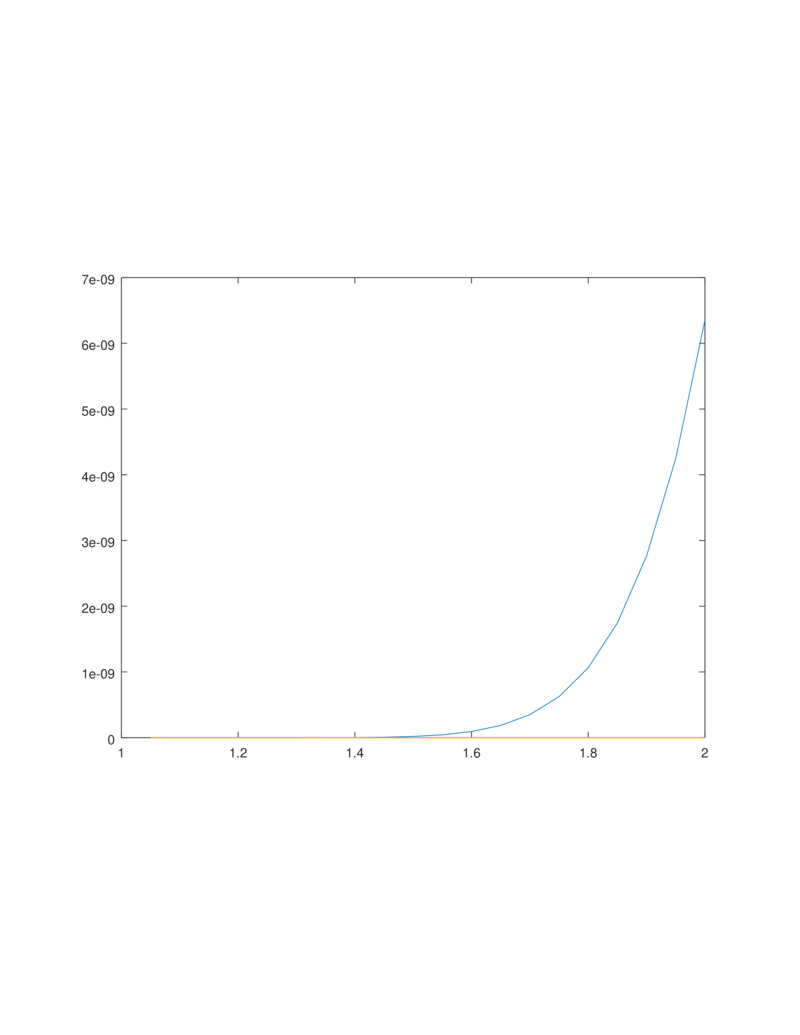
\includegraphics[width=\textwidth]{ln_cf}
  \caption{Relative Error for Continued Fraction Approximation of  $\ln$}
  \label{fig:ln-approx-cf}
\end{figure}

Figure~\ref{fig:ln-approx-taylor} shows the relative approximation error for
$\ln$ with 10, 20, and 50 iterations using a Taylor
series. Figure~\ref{fig:ln-approx-cf} shows the relative approximation error for
10, 20, and 50 iterations using continued fractions. In this case, the error of
the continued fraction approach is multiple orders of magnitude lower for the
same number of iterations.

\begin{figure}[ht]
  \centering
    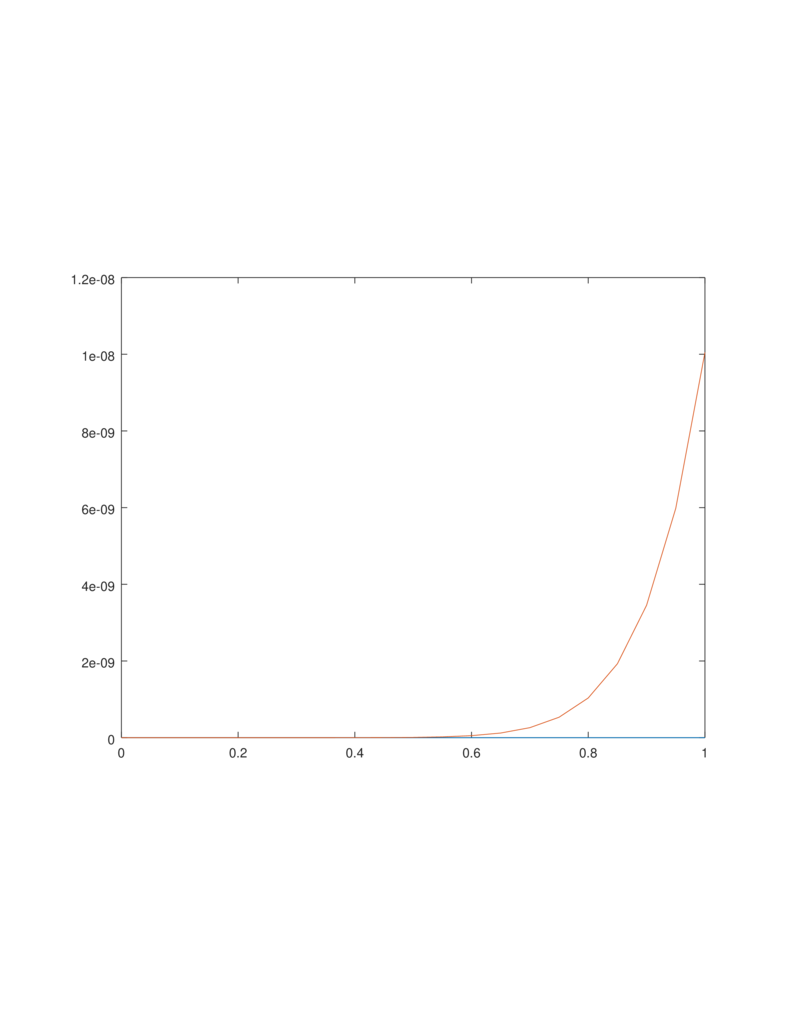
\includegraphics[width=\textwidth]{taylor_exp}
  \caption{Relative Error for Taylor Series Approximation of  $\exp$}
  \label{fig:exp-approx-taylor}
\end{figure}

\begin{figure}[ht]
  \centering
    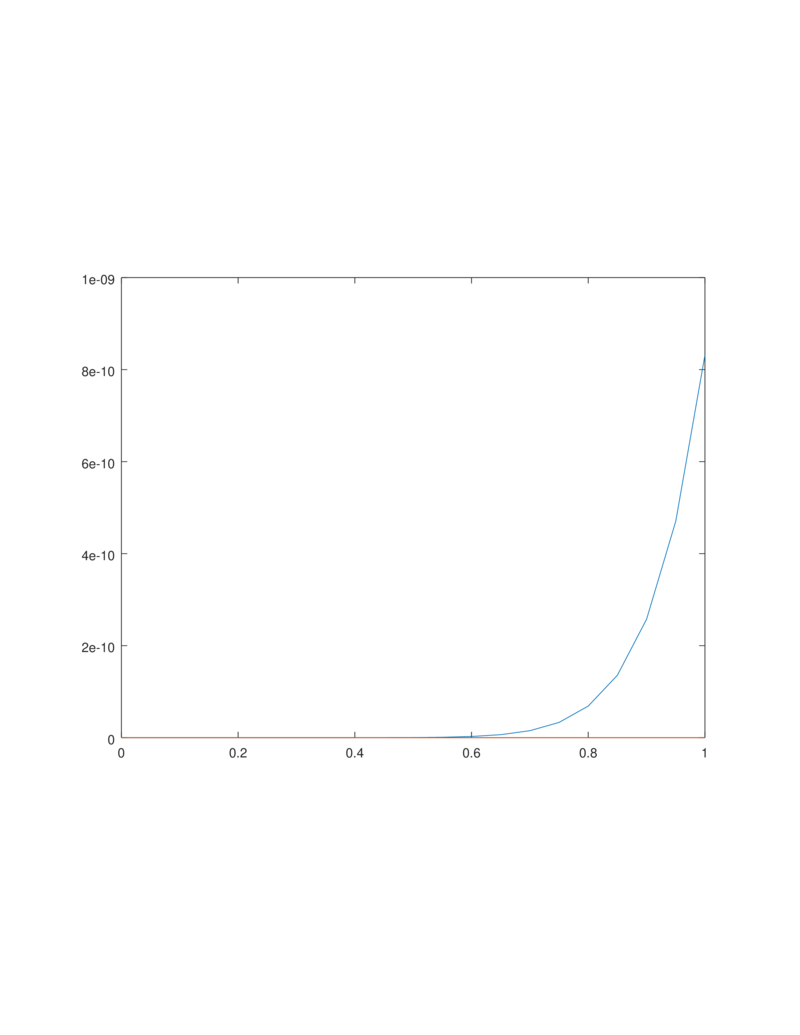
\includegraphics[width=\textwidth]{cf_exp}
  \caption{Relative Error for Continued Fraction Approximation of  $\exp$}
  \label{fig:exp-approx-cf}
\end{figure}

Figure~\ref{fig:exp-approx-taylor} shows the relative approximation error of 10
and 20 iterations using a Taylor series approximation. Figure~\ref{fig:exp-approx-cf}
shows the relative error of 10 and 20 iterations using continued fractions. In
this case the error of continued fractions is around one order of magnitude
lower for the same number of iterations.

\subsection{Conclusion}
\label{sec:conclusion}

From these experiments, we conclude that the convergence speed is higher for
continued fractions, in particular for the natural logarithm algorithm. However,
timing analysis has shown that due to the simpler calculation per iteration of
Taylor series, the exponential function can be approximated more efficiently
using that approach. We have therefore decided to use both approaches: Taylor series for $\exp$
and continued fractions for $\ln$.  In order to decide when the approximation has obtained enough precision,
we use the following criterion for two successive approximations $x_{n}, x_{n+1}$:
\begin{equation*}
  \vert x_{n} - x_{n+1}\vert < \epsilon
\end{equation*}

Both approximation schemes therefore will give the same precision.

\section{Reference Implementation}
\label{sec:refer-impl}

The continued fraction approach using fixed point arithmetic has been
implemented in Haskell and in C using the GNU multi-precision
library~\footnote{\url{https://gmplib.org}}.
%
For the Haskell version, Quickcheck property-based tests are provided that will validate
the mathematical consistency of the laws for $\ln$ and $\exp$.
%
For both the C and Haskell versions, there exist test programs that read
two numbers with 34 decimal digits of precision and calculate
$x^{y}$. This has been used to validate the two different
implementations for 20.000.000 randomly generated testcases, where $x$ and $y$
have been drawn uniformly from the interval $[0.1; 100.1]$. Our results showed that all
calculation were identical for all 34 decimal digits.
A key aspect to obtaining equivalent results is to use the same approach to
rounding after a division. In particular, in our tests we have used rounding to $-\infty$.

\section{Optimisations for Specific Use-Cases}
\label{sec:optim-spec-use}

One specific use case for non-integral calculations in Shelley is the calculation of the
probability of being a slot leader. This calculation has to be done locally every 2s
for each potential slot leader. The calculation also needs to be done in order to
validate a block (to make sure that the block producer actually had the right to
do so).
%
More precisely, it is necessary to check whether for a given $p$, $\sigma$ and a
constant $f$ (at least for one epoch), the following inequality holds:

\begin{equation*}
  p < 1 - {(1 - f)}^{\sigma}
\end{equation*}

Since $1-f$ is considered to be constant, and because ${(1-f)}^{\sigma}$ is equal
to $\exp(\sigma\cdot\ln(1-f))$, we can pre-compute the value of $\ln(1-f)$ once for
each epoch, and use it for every following computation in that epoch.

Setting $c= \ln(1 - f)$ and using $q = 1 - p$ we obtain the following:

\begin{equation*}
  \begin{array}[h]{ccc}
    & p < 1 - \exp(\sigma \cdot c) & \\
    \Leftrightarrow & \exp(\sigma \cdot c) < 1 - p & (\textrm{c is negative})\\
    \Leftrightarrow & \frac{1}{\exp(-\sigma \cdot c)} < q & \\
    \Leftrightarrow & \frac{1}{q} < \exp(-\sigma \cdot c) & \\
    \Leftrightarrow & \ln(\frac{1}{q}) < (-\sigma \cdot c) & \\
    \Leftrightarrow & \ln(q) > \sigma \cdot c &
  \end{array}
\end{equation*}

\noindent
The terms $\exp(-\sigma \cdot c)$ or $\ln(q)$ can be computed using the Taylor series as
described in Section~\ref{sec:taylor-series}.   By using table lookup on $\ln{q}$, a quick
check can be obtained on whether the comparison is definitely true or not true.  If it is
not certain, then the full calculation can be performed. By using a log calculation, integer sizes will
be reduced, which will also improve the performance of the calculation.
Alternatively, since the result of the function falls within known limits, we can use linear lower and upper bounds
to quickly eliminate comparisons that will certainly fail, without needing to perform the full calculation.

Since the relevant information is not the result of the calculation, but only whether
the given $p$ is less than or greater than this value, one can also optimize the $\exp{\ldots}$ or $\ln{\ldots}$
calculation further if desired. Using the Lagrange remainder to estimate the error, it is possible to
only compute as many iterations as necessary to get the desired information.

\begin{equation*}
    T \exp(x; a) := \sum_{n=0}^{\infty}\frac{x^{n}}{n!} =
    \sum_{n=0}^k\frac{x^{n}}{n!} + R_{k}(x)
\end{equation*}

By using an upper bound $M$ on the domain of $x$, the remainder (or error
term) $R_{k}(x)$ can be estimated as follows:

\begin{equation*}
  R_{k}(x) \leq \vert M \cdot \frac{x^{k+1}}{(k+1)!}\vert
\end{equation*}

For the leader election use-case, a good integral bound for the error estimation
is the maximal value of $\vert\ln(1 - f)\vert\leq M$ for $f \in [0, 0.95]$, that
is $M = 3$\footnote{Since $f$ is the active slot coefficient, we will very
  likely stay at lower values, and $M=12$ would then be enough for $[0, 0.99].$}
For larger values of $f$, a different value of $M$ would need to be chosen. The
current value for $f$ in the Shelley ledger is $0.1$.

In general, $M$ can easily be estimated as the smallest
integer that is larger than the exponential function that is evaluated at
the upper bound of the interval of the domain of $x$. For each partial sum $\Sigma_{k}$, it
is then possible to test whether $p$ is greater than $\Sigma_k + \vert R_{k}(x) \vert$ or less than
$\Sigma_k - \vert R_{k}(x)\vert$ in order to decide whether to stop the calculation at an early
iteration.

\begin{figure}[ht]
  \centering
  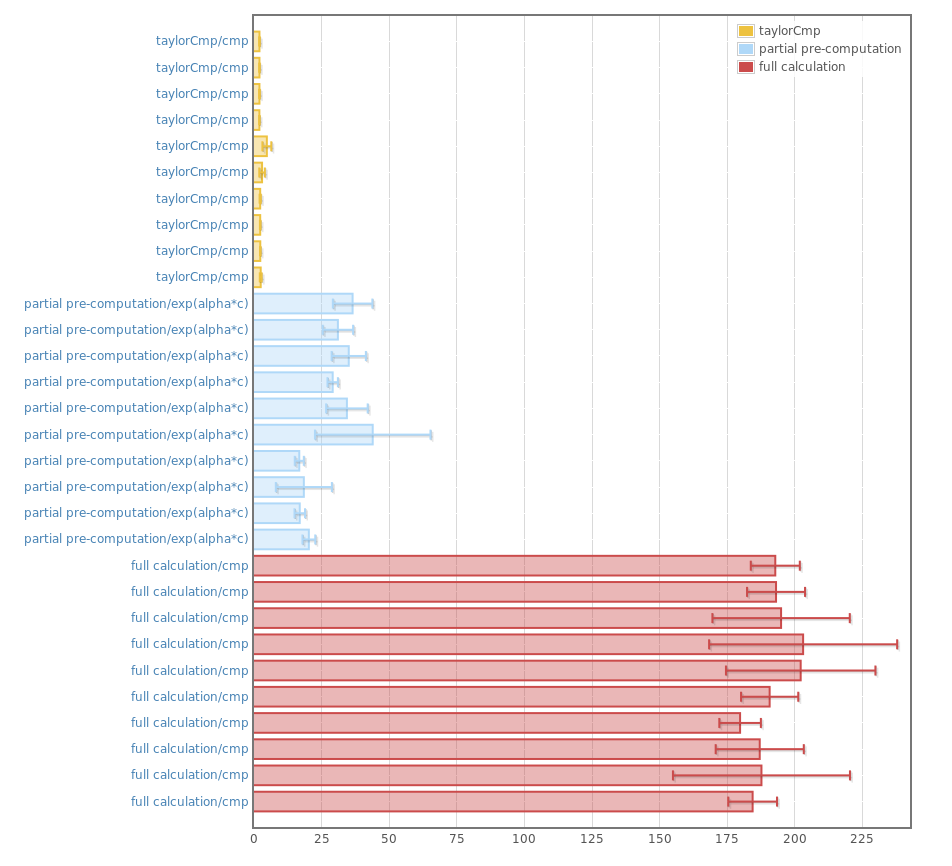
\includegraphics[width=0.75\textwidth]{haskell.png}
  \caption{Benchmark Results for the Haskell Implementation}
  \label{fig:haskell-optimization-results}
\end{figure}

Figure~\ref{fig:haskell-optimization-results} shows the benchmark results for
test data using the Haskell implementation. The lower (red) results show the
run-time (in $\mu s$) for the naive, full computation. The middle (blue) part
shows the run-time using a partial pre-computation of $\ln (1-f)$ for the
exponentiation. The upper (yellow) part shows the run-time using the proposed
optimization. For the 10 data points, the first 5 succeed in the leader
election, the remaining 5 do not.

\addcontentsline{toc}{section}{References}
% \bibliographystyle{plainnat}
\bibliographystyle{habbrv}
\bibliography{references}

\end{document}

%%% Local Variables:
%%% mode: latex
%%% TeX-master: t
%%% End:
